\documentclass{article}
\usepackage{graphicx} 
\usepackage{multicol}
\usepackage{geometry}
\usepackage{amsmath}
\usepackage{booktabs}
\usepackage{pgfplots}
\usepackage{subcaption}
\usepackage[T1]{fontenc}
\usepackage[dvipsnames]{xcolor}
\usepackage{multirow}

\usepgfplotslibrary{statistics}

\geometry{
    left=2cm,
    right=2cm,
    top=2cm,
    bottom=2cm
}

\title{\textbf{Integration Of Deep Learning Into Automatic Cardiovascular Dissection And Reconstruction In Simulated 3D Space For Medical Practice}}
\author{Nguyen Le Quoc Bao \& Le Tuan Hy}
\date{March 2024}

\begin{document}
\maketitle

\begin{center}
\begin{minipage}{0.8\textwidth}
\setlength{\leftskip}{3.5cm} 
\setlength{\rightskip}{3.5cm}
\begin{abstract}
    Accurate and efficient analysis of cardiac images is crucial in the diagnosis and treatment of cardiovascular disease - a leading cause of mortality worldwide and in Vietnam. However, this task is time-consuming, labor-intensive, and prone to errors. The 2D data complicates analysis due to the anatomical complexity and diverse cardiovascular pathologies. Therefore, we have researched and developed the VasculAR software system, integrating deep learning algorithms to fully automate segmentation and reconstruction of 3D cardiac structures from cross-sectional scans; automatically predict 12 cardiovascular diseases; store analysis data on cloud databases; and simulate surgical space for in-depth interactions with cardiac models. We also conducted a study and collected raw cross-sectional cardiac images of Vietnamese patients from Vietnamese hospitals to ensure practical application in our country. We explored 4 deep learning models U-Net, ResUNet, U-Net Attention with 3 loss functions cross entropy (CE), dice loss (DL), and focal loss (FL) for automatic segmentation. Additionally, we investigated the pathologically diagnostic procedure using the Dice Score matching method, and enhanced the speed, accuracy, detail of the 3D reconstruction algorithm. We also developed a virtual reality simulation to assist experts with advanced interactive functions (e.g. slicing, volume/wall thickness measurement) on 3D cardiac structures in virtual reality environment. The resulting Vietnamese heart dataset (VHSCDD) was established; the fully automatic segmentation model Triple View R-Net and 3D cardiac reconstruction algorithm have been affirmed by doctors and experts to facilitate easier observation of cardiac defects. The software system has been tested and evaluated to have high applicability in medical practice and anatomy education. \\
\end{abstract}
\end{minipage}
\end{center}

\begin{multicols}{2} 
\section{Introduction}

\begin{table*}[]
    \centering
    \begin{tabular}{p{2.5cm}|p{2cm}|p{6cm}|p{2.5cm}}
         \textbf{Name} & \textbf{Origin} & \textbf{Description} & \textbf{Cost} \\
         \hline
         VinDir & Vietnam & Analyze bone fractures, spinal injuries, and brain tumors, primarily using 2D X-ray or CT imaging. Not focus on cardiac segmentation and diseases analysis\\
         \hline
         RadiantViewer & Poland & 3D reconstruction model is solid (no segmentation). Observation scope is limited by ribs & $4,733,363$ VNĐ (5 years) \\
         \hline
         ITK-Snap & USA & Manual or semi-automatic segmentation & Free \\
         Materialise & Belgium & Semi-automatic segmentation with human interference & $5,091,240$ VND/month 
    \end{tabular}
    \caption{Existing medical image analysis software}
    \label{tab:1}
\end{table*}

\subsection{Research motivation}
Cardiovascular disease is the leading cause of death globally according to World Health Organization (WHO). About 17.9 million people died from heart disease in 2016 \cite{who}. in Vietnam, cardiovascular disease accounts for 31\% of the causes of death, about more than 170,000 deaths \cite{stanford}. However, 90\% of heart disease can be prevented if diagnosed and detected early \cite{prevent}. Software system supporting analytical and pre-diagnostic work are growing rapidly due to the development of modern medical imaging techniques such as CT and MR \cite{contour}. And \cite{short_axis, left_ventricle, right_ventricle} stated that analysis, evaluation, and reconstruction of cardiac anatomical structures play a huge role in diagnosis, pre-operative planning, early stroke prevention, and disease monitoring \cite{deep_review}. Manual segmentation and analysis by radiologists/physicians is standard in clinical practice \cite{tran, deformable}. However, this work is time-consuming, exhausting, prone to errors \cite{tran, left_ventricle} even infeasible in terms of labour and cost \cite{retrieval}. Currently, traditional  methods (e.g atlas-based/model-based methods) are being applied for semi-automatic segmentation. According to \cite{deep_review}, the advent of Deep Learning has potential to outperform traditional methods in heart tomographic segmentation and. However, the lack of complete data on whole heart segmentation and pathological labeling hinders this development \cite{left_ventricle}. According to \cite{loren}, Three-dimensional anatomical surfaces offer a valuable medical tool by supporting doctors in interpreting complex anatomical structures. Additionally, the exchange of analysis data between radiologists and physicians remains manual and ineffective, hindering treatment planning and post-treatment discussions. Additionally, virtual reality spaces offer enhanced multi-dimensional interactions, potentially revolutionizing anatomy education for medical students.
\subsection{Research objectives}
We define our research objectives as: \\
- Establish a new Vietnamese cardiovascular dataset with 12 segmentation labels with pathological annotations.\\
- Develop a Deep Learning model optimized for proficient performance in cardiac segmentation tasks.\\
- Achieve successful reconstruction of intricate 3D cardiovascular structures. \\
- Implement sophisticated analytical functionalities, including disease diagnosis and cardiac chambers' volume/artery diameter/wall thickness measurement, to support radiologists and physicians in clinical qualitative assessments.\\
- Integrate cloud database into software and incorporate virtual reality technology into simulate surgical environments and enhance interactive experiences.
\subsection{Research Questions}
What criteria define the most suitable and realistic dataset for application in Vietnam? \\
Which deep learning algorithms fully automate the process of segmentation and complete reconstruction of the entire 3D heart? \\
Which diagnostic methods are suitable for CT images and complex cardiovascular structures? \\
How can we enhance clinical assessments by integrating advanced analytical tools into medical imaging software for precise disease diagnosis and quantitative cardiac measurements? \\
What methods enable seamless integration of cloud databases and virtual reality technology into medical software to simulate surgical environments and elevate interactive training experiences for medical professionals? \\

\subsection{Scientific Hypothesis} 
Automating the segmentation and reconstruction process of the 3D heart structure enhances focus on observing the deformation of a specific region/part of the heart, avoiding interference from other parts. Matching algorithms diagnose complex cardiovascular structures appropriately. Deep learning algorithms can learn the intricate structure features of the heart in 3D slice images, minimizing manual preprocessing tasks. Datasets collected from hospitals in Vietnam are the most suitable and realistic for domestic application. Virtual reality environments allow physicians to optimize interaction experiences, enabling them to identify subtle abnormalities not easily discernible in 2D images. Cloud-based databases encrypt information, facilitating patient data management for post-treatment/operative analysis during sessions.

\begin{table*}[]
    \centering
    \begin{tabular}{c|c|c|c|c|c}
         \textbf{Name} & \textbf{Year} & \textbf{Train} & \textbf{Test} & \textbf{Region} & \textbf{P-Labelled} \\
         \midrule
         Sunnybrook & 2009 & 45 & NA & Left ventricle & Yes \\ 
         STACOM &  2011 & 100 & 100 & Left ventricle & No \\ 
         MICCAI RV & 2012 & 16 & 32 & Right ventricle & No \\ 
         ImageTBDA & 2015 & 100 & NA & Aortic duct & Yes \\ 
         MMWHS &  2017 & 40 & 80 & Whole heart (7 regions) & No \\ 
         ImageCAS & 2018 & 1000 & NA & Coronary arteries & Yes \\ 
    \end{tabular}
    \caption{Detailed analysis of current cardiovascular datasets}
    \label{tab:1}
\end{table*}

\subsection{Related Works}
\subsubsection{Existing Medical Data Analysis Software}
See \ref{tab:1} for detailed information. In Vietnam, there's a medical imaging software - VinDir, a website platform with a complete cloud database. However, VinDir doesn't focus on 3D heart reconstruction structures or diagnosing cardiac diseases, and it doesn't employ virtual reality technology. Other software like RadiantViewer, ITK-SNAP is widely used by medical professionals for image analysis, while Materialise is popular in foreign medical facilities. A survey conducted at Hai Duong University of Medicine and Pharmacy with 48 students filling out the survey form shows that Radiant Viewer is the most popular software, at 47.1\%. However, through direct interviews, most students admitted to using unauthorized versions to avoid fees.

\subsection{Existing Cardiac Datasets}
Over the last decade, three international competitions provided distinct datasets. The Sunnybrook Cardiac MR Left Ventricle Segmentation challenge - MICCAI 2009 \cite{left_ventricle} and MICCAI-STACOM 2011 \cite{quantification} focused on left ventricular segmentation, while MICCAI 2012 focused on right ventricular segmentation \cite{right_ventricle}. In 2017, a new competition introduced MMWHS dataset labeling seven heart regions. Additionally, ImageTBDA datasets focus on coronary and aortic artery segmentation, respectively. Research in Vietnam highlights the practicality of segmenting the entire heart due to the complexity of cardiovascular diseases involving multiple adjacent regions. MMWHS is the most comprehensive dataset for training deep learning algorithms, though it lacks detailed disease labeling and intricate structure segmentation, limiting practical applicability, especially in diverse Vietnamese pathologies.

\subsubsection{Deep Learning Models For Cardiac Segmentation}
In 2015, \cite{unet} investigated the U-net model, featuring an Encoder-Decoder architecture, renowned for its effectiveness in image segmentation tasks in biomedical microscopy. In 2016 \cite{tran} pioneered research on Fully Convolutional Neural Networks (FCNs), inheriting the Encoder-Decoder structure to segment the left and right ventricles on MRI images. In 2019, \cite{DenseNets} explored the dense U-Net model with inception modules. In 2018, \cite{attention_unet} proposed the U-net Attention model, capable of noise reduction and focusing on critical parts while training. While this model performed well on the MMWHS dataset, its performance was poor on the new VHSCDD dataset. These models are 2D networks, which are less effective due to their analysis being limited to individual 2D slices within a 3D volume, neglecting the 3D anatomical spatial information. \cite{deep_review}. 

\subsubsection{3D Reconstruction \& Subsequent Qualitative Analysis}
The Marching Cubes algorithm \cite{loren}, proposed by Lorensen in 1987, is commonly used for 3D mesh reconstruction from CT scans. However, it has limitations due to a small lookup table. To address this, Lewiner \cite{lewiner} proposed an improved version with an extended lookup table, resolving the “cracks” issue. This development requires efficient automatic
post analysis, especially measuring important parameters such as volume, surface area, curvature. \cite{limb} presents a system to measure limb volumes using 3D models from an infrared depth sensor. However,
this method does not leverage advanced computed imaging (CT, MR) and may be affected by environmental factors. Intrinsic volume measurement techniques directly from digital 3D images have been explored \cite{intrinsic}, but their computational complexity remains a challenge. 


\section{Methodology}

\begin{figure*}
    \centering
    \includegraphics[width=1\textwidth]{figures/Model Architecture.png}
    \caption{The encoder transforms input into high-level features, while the decoder recovers spatial details from the feature map. Attention mechanism precedes concatenation. The attention gate uses PreLU instead of ReLU for enhanced training. Segmentation results from axial, sagittal, and coronal views are intersected for optimal segmentation}
    \label{fig:1}
\end{figure*}

we established a Vietnamese Heart Segmentation Cardiovascular Dataset (VHSCDD). We developed new robust Deep Learning model for segmentation task named Triple View R-Net (TVRN). We built pathological prognosis procedure with similarity algorithm. We also developed a new algorithm for automatic volume computation directly from volumetric data in 3D reconstruction process with binary indexed tree. Our software system has been distributed to experiment in clinical practice and anatomical education in university.

\subsection{VHSCDD}
Data collection involved obtaining raw CT/CTA slice images from Toshiba Aquilion ONE CT scanner, taken from CT scans of patients between May 2023 and December 2023. Each CT scan produced a 3D image volume with dimensions of $512 \times 600 \times 600$. After acquiring the raw data, preprocessing steps were performed: data anonymization, Hounsfield density processing, and noise removal. Under the guidance and supervision of two cardiologists - Dr. Nguyen Van Nghia, Dr. Le Thi Phuong Nga, and imaging diagnostic expert Dr. Dang Thanh, the team manually segmented 11 detailed parts of the cardiac anatomy using ITK-SNAP: left ventricle, right ventricle, left atrium, right atrium, ascending aorta, aortic arch, superior vena cava, pulmonary artery, myocardium, coronary arteries, and atrioventricular node. Manual segmentation required 4-5 hours per dataset. Results were reviewed and errors corrected weekly from September 2023 to December 2023. A total of 50 successfully segmented datasets, were approved by the validating physicians/radiologists. Cardiac pathology labeling was supervised by Dr. Phuong Nga and verified by Dr. Van Nghia, spanning a two-month period from November 18, 2023 to January 9, 2023.

\subsection{Deep Learning For Segmentation}
\subsubsection{Triple View R-Net}
Traditional 2D networks, such as Unet, often struggle to achieve detailed segmentation in regions of interest due to their limited context awareness. On the other hand, 3D networks, while capable of capturing intricate details, are computationally expensive and challenging to train and deploy in real-world scenarios due to their size and complexity.

To address these challenges, we have developed a novel approach called 2.5D networks called Triple View R-Net (see figure \ref{fig:1}). This network first employ Recurrent Neural Networks (RNNs) to "memorize the past", which allows to propagate contextual information from adjacent slice for better inter-slice coherence. Also, to avoid biases of just one axial view segmentation, our network leverage three view of CT scans (axial, sagittal, coronal", allowing it to capture 3-view spatial connective information. By segmenting on the 3D view and then aggregating the results through intersection, our network produce a most accurate and refined segmentation results compared to others (see figure).

\subsubsection{PReLU Activation Function}
The activation used in attention mechanism of Unet Attention is the non-linear Rectified Linear Unit (ReLU) activation function:
$$ f(y_i) = max(0, y_i) $$
The slope of the negative part is fixed at zero, which can lead to a phenomenon called "dying ReLU" where neurons may become inactive and cease to update their weights. This can slow down or even halt the training process, especially in deeper networks. During the image preprocessing phase, we standardize the volumetric data to the interval $[-1,1]$ to preserve the Hounsfield property. This feature in our input data prompts consideration of replacing the ReLU activation with PReLU. This adjustment helps mitigate the problem of neuron inactivity, resulting in a more resilient and consistent model.

$$ f(y_i) = max(0, y_i) + a \text{min}(0, y_i) $$ 

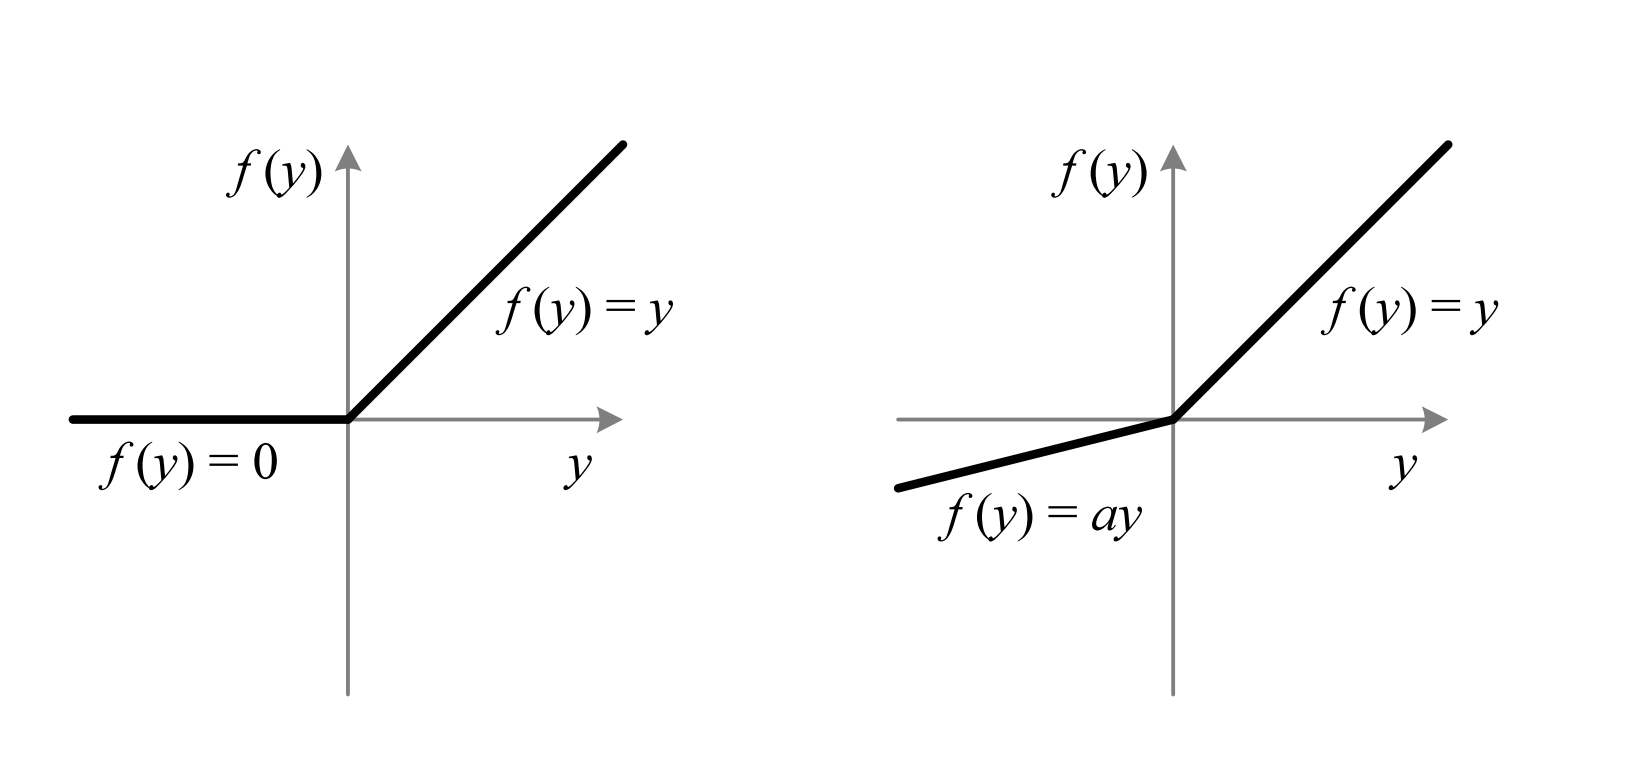
\includegraphics[width=0.48\textwidth]{figures/PReLU.png}



\begin{figure*}
\centering
\begin{subfigure}{0.15\textwidth} % Adjust the width as needed
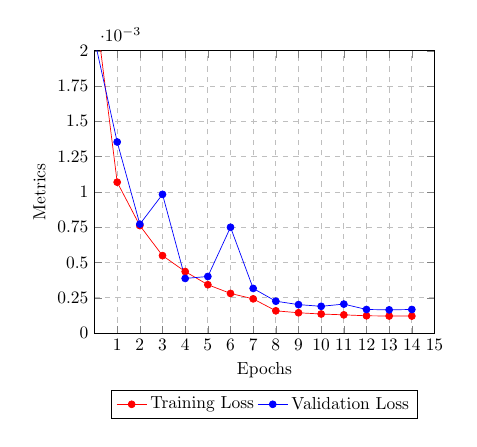
\begin{tikzpicture}[scale=0.63] 
\begin{axis}[
    xlabel={Epochs},
    ylabel={Metrics},
    legend style={at={(0.5,-0.2)},
    anchor=north,legend columns=-1},
    xmin=0, xmax=15,
    ymin=0, ymax=0.002,
    xtick={1,2,3,4,5,6,7,8,9,10,11,12,13,14,15},
    ytick={0.0000,0.00025,0.00050,0.00075,0.00100,0.00125,0.00150,0.00175,0.00200},
    ymajorgrids=true,
    xmajorgrids=true,
    grid style=dashed,
]

% Experiment 1 (gamma=3)
\addplot[color=red,mark=*]
    coordinates {
    (0, 0.0023491743486374617)
    (1, 0.0010687990579754114)
    (2, 0.0007615815848112106)
    (3, 0.0005488840979523957)
    (4, 0.00043598207412287593)
    (5, 0.00034290921757929027)
    (6, 0.00028109399136155844)
    (7, 0.00024261916405521333)
    (8, 0.000157987218699418)
    (9, 0.0001441281638108194)
    (10, 0.00013541760563384742)
    (11, 0.00012942103785462677)
    (12, 0.00012275109475012869)
    (13, 0.00012122908810852095)
(14, 0.00012084362970199436)
    };
\addlegendentry{Training Loss}

\addplot[color=blue,mark=*]
    coordinates {
    (0, 0.0020788467954844236)
    (1, 0.0013535557081922889)
    (2, 0.0007716129184700549)
    (3, 0.0009826284367591143)
    (4, 0.0003873067907989025)
    (5, 0.0004011708952020854)
    (6, 0.0007496534381061792)
    (7, 0.0003165823291055858)
    (8, 0.00022599700605496764)
    (9, 0.00020199039136059582)
    (10, 0.00018989214731846005)
    (11, 0.00020560744451358914)
    (12, 0.0001673449733061716)
    (13, 0.00016490009147673845)
    (14, 0.00016738861449994147)
    };
\addlegendentry{Validation Loss}

\end{axis}
\end{tikzpicture}
\end{subfigure}
\hfill
\begin{subfigure}{0.15\textwidth} % Adjust the width as needed
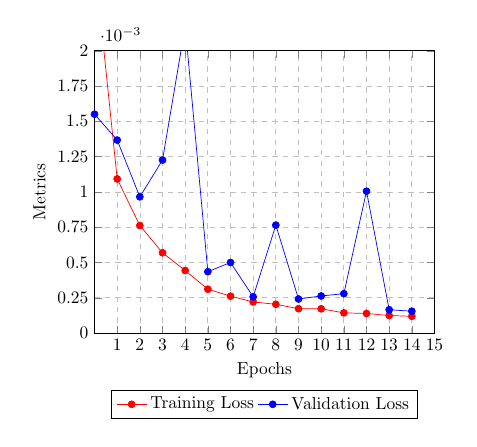
\begin{tikzpicture}[scale=0.63] 
\begin{axis}[
    xlabel={Epochs},
    ylabel={Metrics},
    legend style={at={(0.5,-0.2)},
    anchor=north,legend columns=-1},
    xmin=0, xmax=15,
    ymin=0, ymax=0.002,
    xtick={1,2,3,4,5,6,7,8,9,10,11,12,13,14,15},
    ytick={0.0000,0.00025,0.00050,0.00075,0.00100,0.00125,0.00150,0.00175,0.00200},
    ymajorgrids=true,
    xmajorgrids=true,
    grid style=dashed,
]

% Experiment 2 (gamma=4)
\addplot[color=red,mark=*]
    coordinates {
    (0.0, 0.0026418539540221)
    (1.0, 0.0010919938407217)
    (2.0, 0.0007622729754074666)
    (3.0, 0.0005692125705536)
    (4.0, 0.00044349951591956665)
    (5.0, 0.00031100302779419996)
    (6.0, 0.0002620883121077)
    (7.0, 0.00022069115463326666)
    (8.0, 0.0002041034895227667)
    (9.0, 0.00017322452913496664)
    (10.0, 0.0001722997840260667)
    (11.0, 0.00014349746682755903)
    (12.0, 0.00013915516804745284)
    (13.0, 0.000124861056974607)
    (14.0, 0.00011895461648236303)
    };
\addlegendentry{Training Loss}

\addplot[color=blue,mark=*]
    coordinates {
    (0.0, 0.0015502179351945002)
    (1.0, 0.0013671716442331002)
    (2.0, 0.0009648650302551)
    (3.0, 0.0012257071211933333)
    (4.0, 0.002174725076959733)
    (5.0, 0.00043520538019943333)
    (6.0, 0.0005000755578899999)
    (7.0, 0.0002570857808071)
    (8.0, 0.0007649362378287335)
    (9.0, 0.00024165183519166667)
    (10.0, 0.00026311726348163337)
    (11.0, 0.0002794276321461667)
    (12.0, 0.0010049991954777357)
    (13.0, 0.00016561815088300758)
    (14.0, 0.00015532811084992826)
    };
\addlegendentry{Validation Loss}

\end{axis}
\end{tikzpicture}
\end{subfigure}
\hfill
\begin{subfigure}{0.3\textwidth}
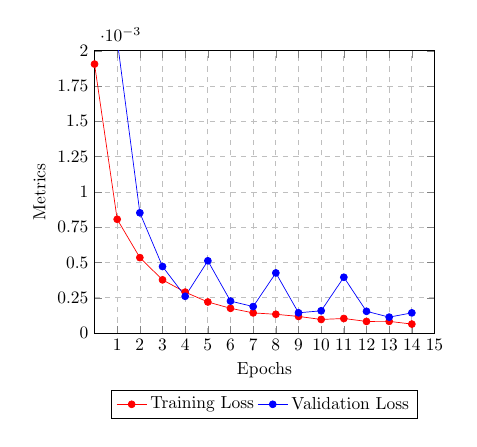
\begin{tikzpicture}[scale=0.63] 
\begin{axis}[
    xlabel={Epochs},
    ylabel={Metrics},
    legend style={at={(0.5,-0.2)},
    anchor=north,legend columns=-1},
    xmin=0, xmax=15,
    ymin=0, ymax=0.002,
    xtick={1,2,3,4,5,6,7,8,9,10,11,12,13,14,15},
    ytick={0.0000,0.00025,0.00050,0.00075,0.00100,0.00125,0.00150,0.00175,0.00200},
    ymajorgrids=true,
    xmajorgrids=true,
    grid style=dashed,
]

% Experiment 3 (gamma=5)
\addplot[color=red,mark=*]
    coordinates {
    (0, 0.0019051628187298775)
    (1, 0.0008063178393058479)
    (2, 0.0005347100086510181)
    (3, 0.0003772639320231974)
    (4, 0.00029033111059106886)
    (5, 0.00022059143520891666)
    (6, 0.00017572801152709872)
    (7, 0.00014333620492834598)
    (8, 0.00013341235171537846)
    (9, 0.000118262178148143)
    (10, 9.679690265329555e-05)
    (11, 0.00010362754255766049)
    (12, 8.284807699965313e-05)
    (13, 8.340533531736583e-05)
    (14, 6.411522917915136e-05)
    };
\addlegendentry{Training Loss}

\addplot[color=blue,mark=*]
    coordinates {
    (0, 0.0020657044369727373)
    (1, 0.0020744907669723034)
    (2, 0.0008521018899045885)
    (3, 0.00047188103781081736)
    (4, 0.0002609254152048379)
    (5, 0.0005121429567225277)
    (6, 0.00022683355200570077)
    (7, 0.00018813714268617332)
    (8, 0.0004264016170054674)
    (9, 0.00014395223115570843)
    (10, 0.00015817485109437257)
    (11, 0.0003957666631322354)
    (12, 0.000154521971126087)
    (13, 0.00011323890066705644)
    (14, 0.0001434599980711937)
    };
\addlegendentry{Validation Loss}
\end{axis}
\end{tikzpicture}
\end{subfigure}
\caption{Loss values on different gamma values}
\end{figure*}

\begin{figure*}
\centering
\begin{subfigure}{0.15\textwidth} % Adjust the width as needed
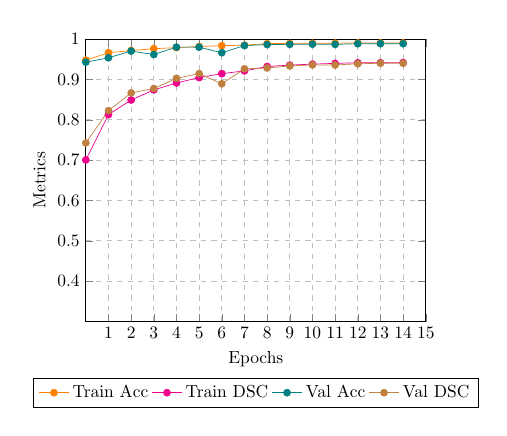
\begin{tikzpicture}[scale=0.63] 
\begin{axis}[
    xlabel={Epochs},
    ylabel={Metrics},
    legend style={at={(0.5,-0.2)},
    anchor=north,legend columns=-1},
    xmin=0, xmax=15,
    ymin=0.3, ymax=1,
    xtick={1,2,3,4,5,6,7,8,9,10,11,12,13,14,15},
    ytick={0.4,0.5,0.6,0.7,0.8,0.9,1},
    ymajorgrids=true,
    xmajorgrids=true,
    grid style=dashed,
]

% Experiment 1 (gamma=3)
\addplot[color=orange,mark=*]
    coordinates {
    (0, 0.9476693868637085)
    (1, 0.9661701917648315)
    (2, 0.9716621041297913)
    (3, 0.9761903285980225)
    (4, 0.9788916707038879)
    (5, 0.9815940260887146)
    (6, 0.9836104512214661)
    (7, 0.985001266002655)
    (8, 0.9887281060218811)
    (9, 0.9893127679824829)
    (10, 0.9896594285964966)
    (11, 0.9899787306785583)
    (12, 0.9903295040130615)
    (13, 0.9903799891471863)
    (14, 0.9904184341430664)
    };
\addlegendentry{Train Acc}

\addplot[color=magenta,mark=*]
    coordinates {
    (0, 0.7005423903465271)
    (1, 0.8129056692123413)
    (2, 0.849026620388031)
    (3, 0.8740505576133728)
    (4, 0.8911991715431213)
    (5, 0.9046808481216431)
    (6, 0.9143446087837219)
    (7, 0.9212019443511963)
    (8, 0.9320273995399475)
    (9, 0.9355268478393555)
    (10, 0.9380083084106445)
    (11, 0.9399060606956482)
    (12, 0.9412676095962524)
    (13, 0.9415480494499207)
    (14, 0.9417922496795654)
    };
\addlegendentry{Train DSC}

\addplot[color=teal,mark=*]
    coordinates {
    (0, 0.9428954720497131)
    (1, 0.9535948634147644)
    (2, 0.9702972769737244)
    (3, 0.9617093801498413)
    (4, 0.9802038073539734)
    (5, 0.9799967408180237)
    (6, 0.9662241339683533)
    (7, 0.9840244054794312)
    (8, 0.986379086971283)
    (9, 0.9870290160179138)
    (10, 0.9874100089073181)
    (11, 0.9869822263717651)
    (12, 0.9885097742080688)
    (13, 0.9886946678161621)
    (14, 0.9886072874069214)
    };
\addlegendentry{Val Acc}

\addplot[color=brown,mark=*]
    coordinates {
    (0, 0.7426415681838989)
    (1, 0.8226363062858582)
    (2, 0.8665981888771057)
    (3, 0.8774776458740234)
    (4, 0.9027673602104187)
    (5, 0.9145081043243408)
    (6, 0.8892216682434082)
    (7, 0.9262991547584534)
    (8, 0.9284138083457947)
    (9, 0.9335697889328003)
    (10, 0.9360981583595276)
    (11, 0.9359386563301086)
    (12, 0.9387704730033875)
    (13, 0.9402453303337097)
    (14, 0.9400850534439087)
    };
\addlegendentry{Val DSC}

\end{axis}
\end{tikzpicture}
\end{subfigure}
\hfill
\begin{subfigure}{0.15\textwidth} % Adjust the width as needed
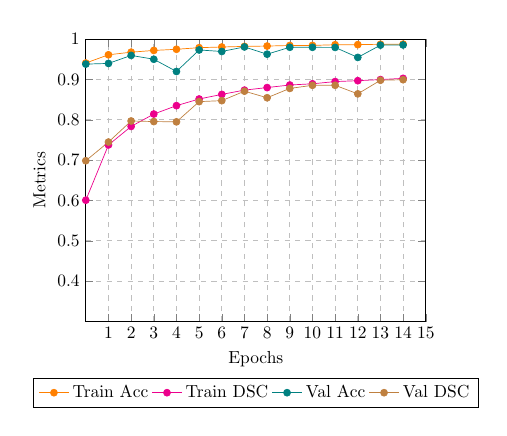
\begin{tikzpicture}[scale=0.63] 
\begin{axis}[
    xlabel={Epochs},
    ylabel={Metrics},
    legend style={at={(0.5,-0.2)},
    anchor=north,legend columns=-1},
    xmin=0, xmax=15,
    ymin=0.3, ymax=1,
    xtick={1,2,3,4,5,6,7,8,9,10,11,12,13,14,15},
    ytick={0.4,0.5,0.6,0.7,0.8,0.9,1},
    ymajorgrids=true,
    xmajorgrids=true,
    grid style=dashed,
]

% Experiment 2 (gamma=4)
\addplot[color=orange,mark=*]
    coordinates {
    (0.0, 0.9407186508178711)
    (1.0, 0.9611082077026367)
    (2.0, 0.9675916433334351)
    (3.0, 0.9718948403994242)
    (4.0, 0.9747803608576456)
    (5.0, 0.9787723819414774)
    (6.0, 0.9803751905759176)
    (7.0, 0.9819322625796)
    (8.0, 0.9827885429064432)
    (9.0, 0.9841493566830953)
    (10.0, 0.9843512773513794)
    (11.0, 0.9860418637593588)
    (12.0, 0.986237366994222)
    (13.0, 0.987195611000061)
    (14.0, 0.9875624577204386)
    };
\addlegendentry{Train Acc}

\addplot[color=magenta,mark=*]
    coordinates {
    (0.0, 0.6006728013356527)
    (1.0, 0.7376534541447958)
    (2.0, 0.7835755149523417)
    (3.0, 0.8142380913098654)
    (4.0, 0.8350525697072347)
    (5.0, 0.8515606919924418)
    (6.0, 0.8629716237386068)
    (7.0, 0.8735610445340475)
    (8.0, 0.8798799514770508)
    (9.0, 0.8862309058507284)
    (10.0, 0.8892091711362203)
    (11.0, 0.8947319587071737)
    (12.0, 0.896936813990275)
    (13.0, 0.8996868332227071)
    (14.0, 0.902715007464091)
    };
\addlegendentry{Train DSC}

\addplot[color=teal,mark=*]
    coordinates {
    (0.0, 0.9380459785461426)
    (1.0, 0.939689020315806)
    (2.0, 0.9595901568730673)
    (3.0, 0.9500625133514404)
    (4.0, 0.91973348458608)
    (5.0, 0.9730887611707052)
    (6.0, 0.9693205157915751)
    (7.0, 0.980548620223999)
    (8.0, 0.9626035094261169)
    (9.0, 0.9797592361768087)
    (10.0, 0.9796677430470785)
    (11.0, 0.9793954094250997)
    (12.0, 0.9546082417170206)
    (13.0, 0.9850619236628214)
    (14.0, 0.9855313102404276)
    };
\addlegendentry{Val Acc}

\addplot[color=brown,mark=*]
    coordinates {
    (0.0, 0.6985171834627787)
    (1.0, 0.7448277076085409)
    (2.0, 0.7970297733942667)
    (3.0, 0.7956840395927429)
    (4.0, 0.794929047425588)
    (5.0, 0.8450055321057638)
    (6.0, 0.8474732438723246)
    (7.0, 0.8709048827489217)
    (8.0, 0.8546351591746012)
    (9.0, 0.8777625759442648)
    (10.0, 0.8854535619417826)
    (11.0, 0.8854933579762777)
    (12.0, 0.8643035888671875)
    (13.0, 0.8980056643486023)
    (14.0, 0.8993767897288004)
    };
\addlegendentry{Val DSC}

\end{axis}
\end{tikzpicture}
\end{subfigure}
\hfill
\begin{subfigure}{0.3\textwidth}
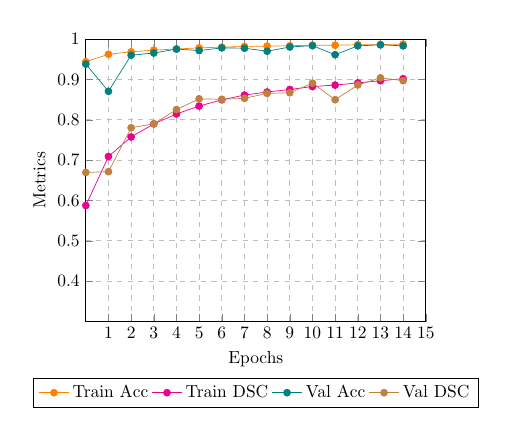
\begin{tikzpicture}[scale=0.63] 
\begin{axis}[
    xlabel={Epochs},
    ylabel={Metrics},
    legend style={at={(0.5,-0.2)},
    anchor=north,legend columns=-1},
    xmin=0, xmax=15,
    ymin=0.3, ymax=1,
    xtick={1,2,3,4,5,6,7,8,9,10,11,12,13,14,15},
    ytick={0.4,0.5,0.6,0.7,0.8,0.9,1},
    ymajorgrids=true,
    xmajorgrids=true,
    grid style=dashed,
]

% Experiment 3 (gamma=5)
\addplot[color=orange,mark=*]
    coordinates {
    (0, 0.9439168572425842)
    (1, 0.9623996019363403)
    (2, 0.9684903621673584)
    (3, 0.9726738929748535)
    (4, 0.9754011631011963)
    (5, 0.9782773852348328)
    (6, 0.980076014995575)
    (7, 0.9818074703216553)
    (8, 0.9826061725616455)
    (9, 0.9835513234138489)
    (10, 0.9850081205368042)
    (11, 0.9848687648773193)
    (12, 0.9860573410987854)
    (13, 0.9864388108253479)
    (14, 0.9877020716667175)
    };
\addlegendentry{Train Acc}

\addplot[color=magenta,mark=*]
    coordinates {
    (0, 0.5875736474990845)
    (1, 0.7090553641319275)
    (2, 0.7574641704559326)
    (3, 0.7897876501083374)
    (4, 0.8144261837005615)
    (5, 0.8340877294540405)
    (6, 0.8495032787322998)
    (7, 0.8612955212593079)
    (8, 0.8688181638717651)
    (9, 0.8751410245895386)
    (10, 0.8823495507240295)
    (11, 0.8860716819763184)
    (12, 0.8914124965667725)
    (13, 0.8967520594596863)
    (14, 0.9019237756729126)
    };
\addlegendentry{Train DSC}

\addplot[color=teal,mark=*]
    coordinates {
    (0, 0.9379929900169373)
    (1, 0.8705695867538452)
    (2, 0.9600841999053955)
    (3, 0.9655229449272156)
    (4, 0.9752795696258545)
    (5, 0.9715473055839539)
    (6, 0.978225827217102)
    (7, 0.9774079918861389)
    (8, 0.970018208026886)
    (9, 0.9803858995437622)
    (10, 0.9837945103645325)
    (11, 0.9612416625022888)
    (12, 0.9832207560539246)
    (13, 0.9857977032661438)
    (14, 0.9832888841629028)
    };
\addlegendentry{Val Acc}

\addplot[color=brown,mark=*]
    coordinates {
    (0, 0.6694716215133667)
    (1, 0.6714617609977722)
    (2, 0.7803776860237122)
    (3, 0.7900828719139099)
    (4, 0.8252691030502319)
    (5, 0.8519533276557922)
    (6, 0.8508435487747192)
    (7, 0.8530938625335693)
    (8, 0.8654612302780151)
    (9, 0.8670518398284912)
    (10, 0.8908647298812866)
    (11, 0.8497445583343506)
    (12, 0.8863067626953125)
    (13, 0.9039372801780701)
    (14, 0.8969414830207825)
    };
\addlegendentry{Val DSC}


\end{axis}
\end{tikzpicture}
\end{subfigure}
\caption{Accuracy (Acc) \& Dice Coefficient Score (DSC) with different $\gamma$ values}
\end{figure*}

\subsubsection{Loss Function}
nitially, our experimentation focused on employing the cross entropy loss and Dice Loss functions:
$$ \text{Dice Loss} = 1 - \frac{{2 \times \sum_{i}^{N} y_i \times p_i}}{{\sum_{i}^{N} y_i + \sum_{i}^{N} p_i}} $$
Although the intial training accuracy was high, the segmentation results were suboptimal for critical classes like coronary arteries. The model struggled to discern areas needing focus, particularly in distinguishing foreground from background. This led to inflated accuracy metrics but inefficiencies in segmentation, particularly due to facile background classification. Consequently, we addressed the inherent class imbalance issue by implementing the focal loss  function.

The focal loss is initialized from the cross entropy (CE) loss for binary classification
$$
\text{CE}(p,y) = 
\left\{
\begin{array}{ll}
    -\text{log}(p) & \text{if } y=1 \\
    -\text{log}(1-p) & \text{otherwise} \\
\end{array}
\right.
$$

In above $y \in {\pm 1}$ specifies the ground-truth class and $p \in [0,1]$ is the model's estimated probability for the class with label $y=1$. For notational convenience, \cite{focal} define $p_t$ as:

$$
p_t = 
\left\{
\begin{array}{ll}
    p & \text{if } y=1 \\
    1 - p & \text{otherwise} \\
\end{array}
\right.
$$

The large class imbalance encountered during training procedure of Deep Learning models overwhelms the cross entropy loss. Easily classified negatives (black background in our case) comprise the majority of loss and dominate the gradient, leading to the high accuracy and minimal loss while training but major misclassification of important regions/details. Therefore, the incorporated focal loss can help by down-weighting easy examples and thus focus training on hard negatives. This loss function is defined by adding factor $f=(1-p_t)$ to the cross entropy loss with tunable focusing parameter $\gamma$:


$$   f = (1-p_t)^{\gamma} $$
$$  \text{FL}(p_t) = -f log(p_t) $$


In our training process, the background, occupying the most spatial pixels in volumetric data, is the easy examples. This $12_th$ class not only contribute no useful learning signal but also degenerate our model. When this class is well-classified or $p_t \rightarrow 1$, the modulating factor $f \rightarrow 0$ and the loss for this class is down-weighted. Inversely, the coronary artery is the most difficult region for our model to classify. When this region is misclassified or $p_t \rightarrow 0$, the $f \rightarrow 1$ and the loss is unaffacted. By setting $\gamma > 1$, we can increase the loss for examples that are misclassified with high confidence. We found $\gamma = 5$ work best in our experiment (see figure 3). \\

\subsubsection{Comparison}
We conducted experiments utilizing various neural network architectures, including Unet, Unet Attention, ResUnet, and VAS, utilizing the GPU RTX 4090. The average dice score was calculated for each model across 12 segmentation regions. Our findings reveal that our VAS model consistently outperforms the other architectures in terms of segmentation accuracy and performance. 

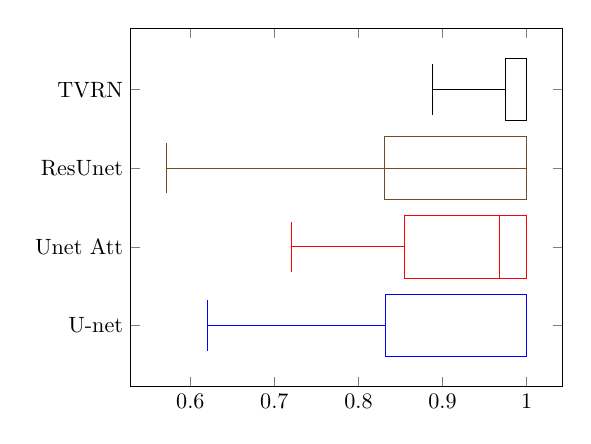
\begin{tikzpicture}[scale=0.8]
    \begin{axis}
      [
      ytick={1,2,3,4},
      yticklabels={U-net, Unet Att, ResUnet, TVRN}, 
      ]
      \addplot+[
      boxplot prepared={
        median=0.999987,
        upper quartile=1,
        lower quartile=0.832546,
        upper whisker=1.0,
        lower whisker=0.6204703875
      },
      ] coordinates {};
      \addplot+[
      boxplot prepared={
        median=0.967956,
        upper quartile=1.0,
        lower quartile=0.8550402,
        upper whisker=1.0,
        lower whisker=0.7200176891666668
      },
      ] coordinates {};
      \addplot+[
      boxplot prepared={
        median=1,
        upper quartile=0.831131,
        lower quartile=1,
        upper whisker=1.0,
        lower whisker=0.5719854583333334
      },
      ] coordinates {};
      \addplot+[
      boxplot prepared={
        median=1,
        upper quartile=1,
        lower quartile=0.9743816,
        upper whisker=1.0,
        lower whisker=0.88749311
      },
      ] coordinates {};
    \end{axis}
\end{tikzpicture} \\
Figure: Average Dice Score over 12 regions of 4 models \\


\subsection{Pathological Diagnosis}
\subsubsection{Similarity-based method} 
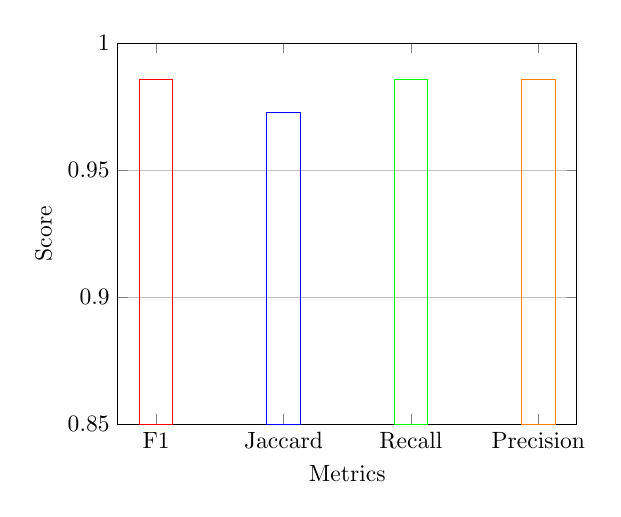
\begin{tikzpicture}[scale=0.85]
    \begin{axis}[
        xlabel={Metrics},
        ylabel={Score},
        bar width=0.5cm,
        symbolic x coords={F1,Jaccard,Recall,Precision}, 
        xtick={F1,Jaccard,Recall,Precision},
        ymajorgrids,
        ymin=0.85, ymax=1,
        ]
        \addplot[ybar, fill=none, draw=red] coordinates {
        (F1, 0.9857923996)  
        };
        \addplot[ybar, fill=none, draw=blue] coordinates {
        (Jaccard, 0.9727066629)
        };
        \addplot[ybar, fill=none, draw=green] coordinates {
        (Recall, 0.9857923996)
        };
        \addplot[ybar, fill=none, draw=orange] coordinates {
        (Precision, 0.9857923996) 
        };
    \end{axis}
\end{tikzpicture}

Diagnosing diseases from images mainly uses bounding boxes or multi-layer classification with input from 2D images, commonly X-ray images. However, with 3D images such as CT and MRI, which include many 2D image slices, which slice must we choose to predict any disease? For example, the coronary artery appears from slice number 200-230 in CT image set 1 and from slice number 265-270 in CT image set 2, and only 1-2 slices have abnormal signs, we How should the bounding box be trained if each coronary artery slice moves the structure in space? The team tested the above method and failed at the training step. Multi-class image classification is even more impossible because the CT image set is a very complex 3D block, not as simple as classifying simple dog or cat images. Thus, the group uses the similarity comparison method. Diagnostic process in chart 13: When there are segmentation results from the VAS model, the algorithm separates and stores 11 different regions using a filtering array of 11 different pixel values to get each separate part. Then, the user selects the pathology they want to diagnose (12 pathologies) and the algorithm will select the parts that need to be analyzed. For example, when diagnosing patent ductus arteriosus, the aortic arch and pulmonary artery will be selected for analysis. Next, these two parts will be used to compare using Dice Coefficient Score with the pulmonary arteries and aortic arch of the data sets labeled with patent ductus arteriosus and those without patent ductus arteriosus. circuit. The result of disease or normal (percentage) is the average of the above Dice Score values.




\subsection{3D cardiac reconstruction}
\includegraphics[width=0.5\textwidth]{figures/3d DIS.png} \\
Figure: 3D reconstruction examples of 12 cardiac pathologies \\

The Marching Cubes is uses the divide-and-conquer approach to locate the surface in logical cubes created from eight pixels; four each from two adjacent slices. In medical image, the cube is usually considered a voxel with predetermined ratio to real world unit. In three dimensional space, the relationship between a voxel and the 3D object mesh is classified into three cases: the voxel is totally inside the mesh, partly intersected by the surface mesh, or totally located outside the mesh. The surface can intersect the voxel in $2^8=256$ cases since a voxel has $8$ vertices in total (this can be proved by generation method). \\


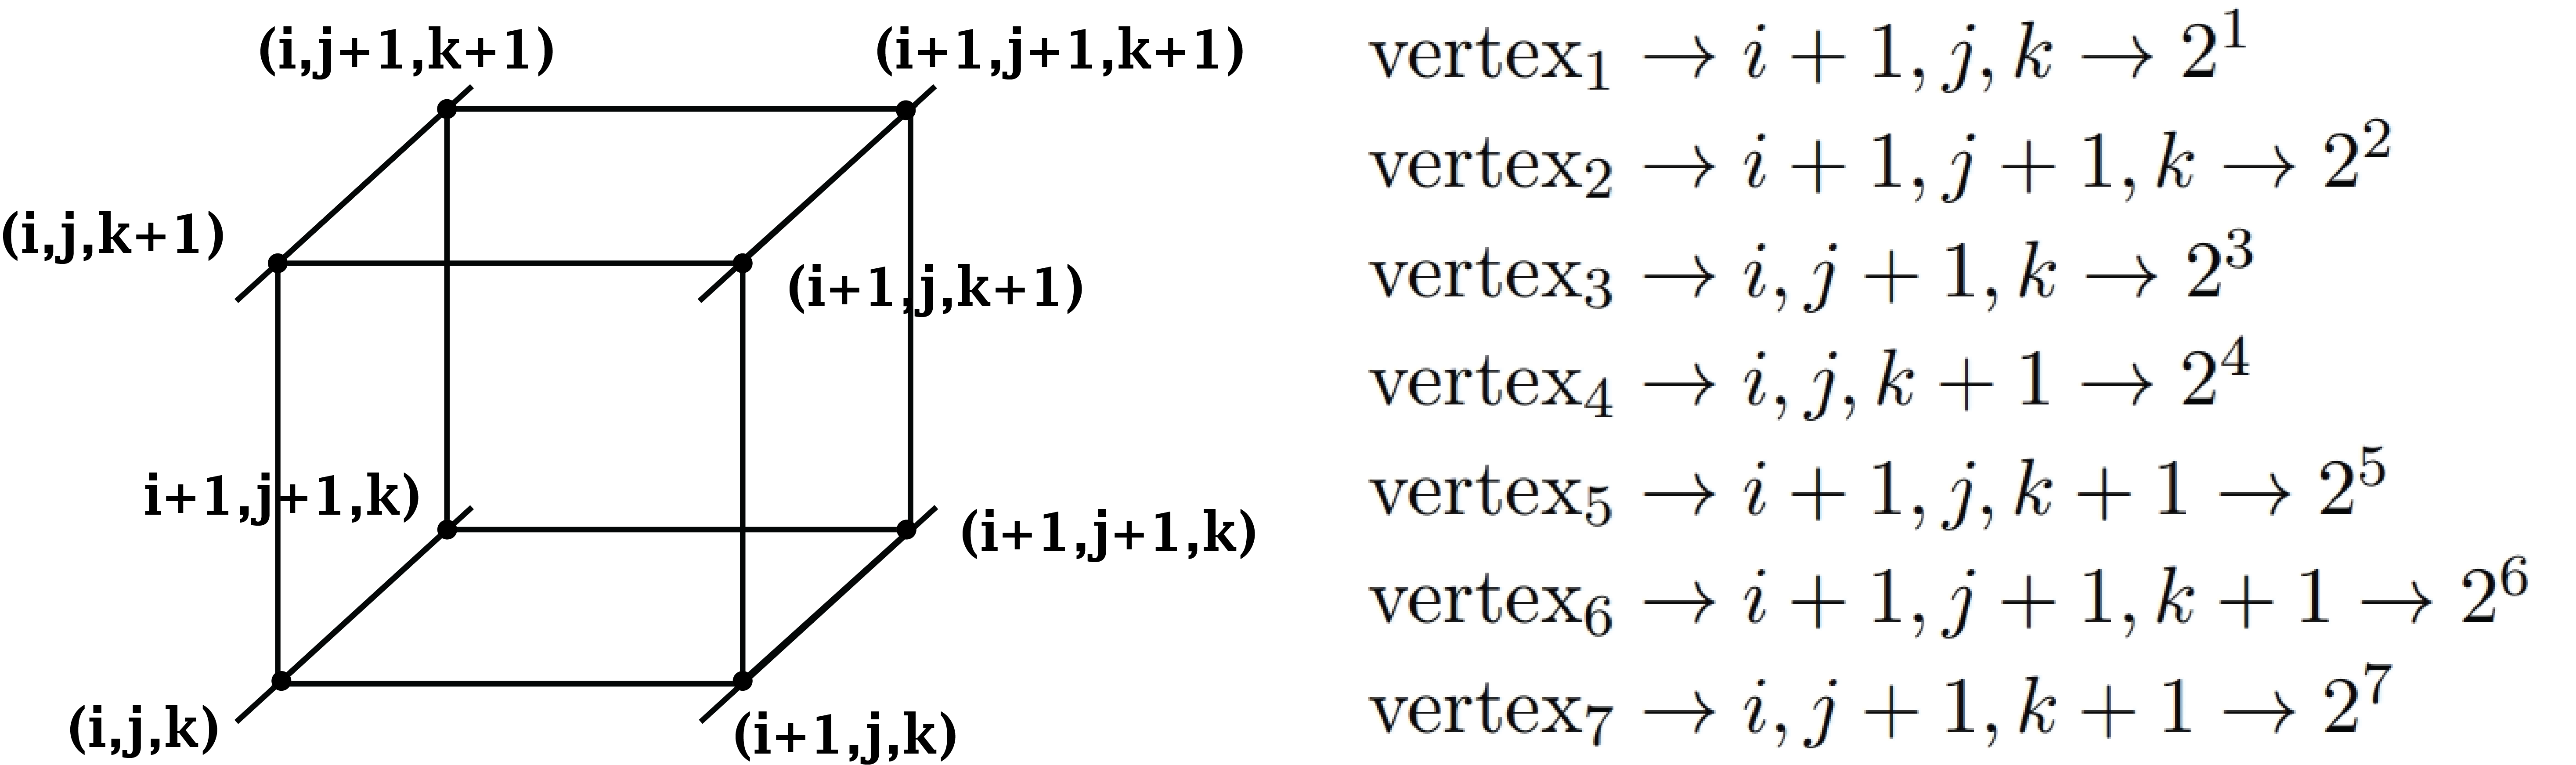
\includegraphics[width=0.48\textwidth]{figures/Binary Vertices.png}
Figure: Vertex indexing and binary representation \\

The reduced problem from 256 cases to 14 patterns is can be achieved thanks to symmetrical property and rotational symmetry. From original 3D array, the algorithm create the boolean 3D array with the same size speculating that a vertex is false if locates inside the model and vice versa. 

\subsubsection{Resolving Topologically Accuracy Issues}
The algorithm can lead to cracks because the same configuration can be tiled in different way. Therefore we researched and applied a more efficient implementation with extended lookup table proposed by Lewiner with 32 base cases to ensure the topologically correction reconstruction of detailed and sensitive cardiac regions such as coronary arterties and heart capillaries.

The algorithm under consideration is typically employed in processing raw volumetric data to extract isosurfaces using a customizable thresholding parameter. Its primary function is to meticulously represent the features present in the raw data. However, in certain cases such as chest CT scans, the presence of ribs can obstruct the observation of internal cardiac structures. To address this, we utilize the segmentation results obtained from the Triple View R-net to generate a binary image, which is then used to reconstruct individual components. Due to the binary nature of the pixel values (either 1 or 0), employing a threshold of 0.5 fails to produce finely triangulated and topologically accurate structures. To overcome this limitation, we propose a hybrid method that utilizes the segmentation results as a filter mask for the original raw data.

Mathematically, this can be expressed as:
$$F, D, B \in {R}^{N \times M \times P} : F = D \odot B$$

where $D$ represents the volumetric data, $B$ denotes the binary image, and $F$ signifies the filtered result.

\subsubsection{Resolving Speed Issues}
The marching cubes algorithm iterates through three-dimensional axes (ox, oy, oz) with a time complexity of $O(N \times M \times P)$, where $N, M, P$ correspond to the dimensions of the dataset. To enhance computational efficiency, we have implemented the algorithm using Cython, a Python-to-C compiler known for its efficiency in code optimization. This approach significantly accelerates the volume rendering process, enabling us to achieve both precision and computational speed simultaneously.The average reconstruction speed for each component is consistently below 5 seconds, totaling 55 seconds for all 11 parts. Subsequently, the reconstruction results are stored in STL/OBJ file formats within a cloud-based database, facilitating seamless access and utilization within virtual environments.


\subsection{Subsequent Quantitative Cardiac Analysis}

To ensure the meticulous measurement and analysis of intricate 3D structures with utmost accuracy and efficiency \cite{intrinsic}. Of particular significance is the quantification of various parameters within the cardiovascular system, including but not limited to the diameter, area, and volume of critical structures such as the aortic duct. These metrics serve as crucial indicators for pathologies such as hypertrophy or stenosis, which pose significant risks to patient well-being. Consequently, the accurate assessment and preoperative planning facilitated by such analyses substantially enhance the clinical efficacy and safety of surgical interventions. 

\subsubsection{Volume Computation with Triple Integral \& Binary Indexed Tree}

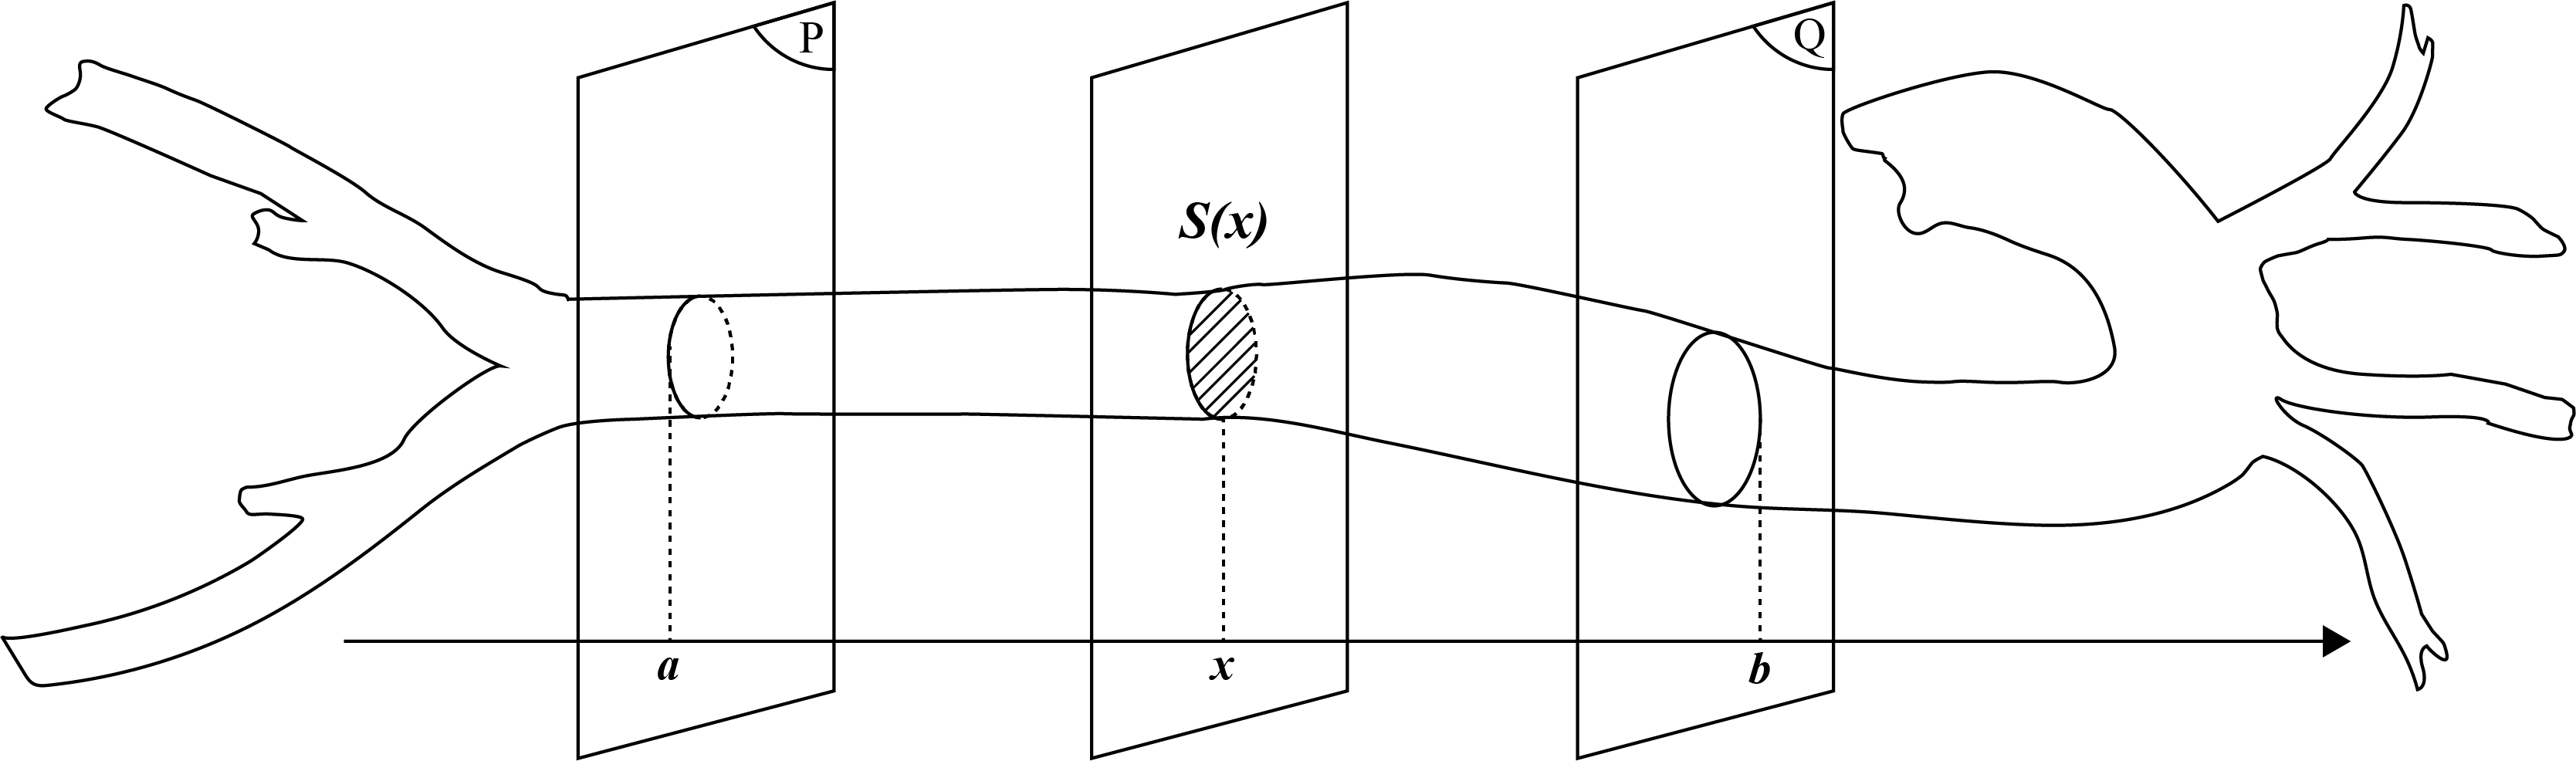
\includegraphics[width=0.45\textwidth]{figures/Integral Surface Function.png} \\
Figure: Integral idea to calculate the volume

$$
\iiint_V f(x, y, z) \, dx \, dy \, dz
$$

Combining multivariable calculus, marching cubes algorithm, and binary indexed tree data structure, we develop a algorithm for efficient computation of intrinsic volume. We proposed the 30 configurations of volume values based on polygonal mesh generation method. Our algorithm processes the data in scan-line order to initialize the Fenwick tree simultaneously with the reconstruction algorithm, ensuring faster volume query time following users edition such as slicing or transforming object mesh. We utilize the 3D Fenwick tree (developed from the original 1D Fenwick tree \cite{fenwick}). With this data structure, we can achieve the time complexity $O(Q \times log(N) \times log(M) \times log(P))$ instead of $O (Q \times N \times M \times P)$ with $Q$ is the number of query (e.g slicing, mesh edition) by user and $N,M,P$ is the 3 dimensional of volumetric data correspondingly.

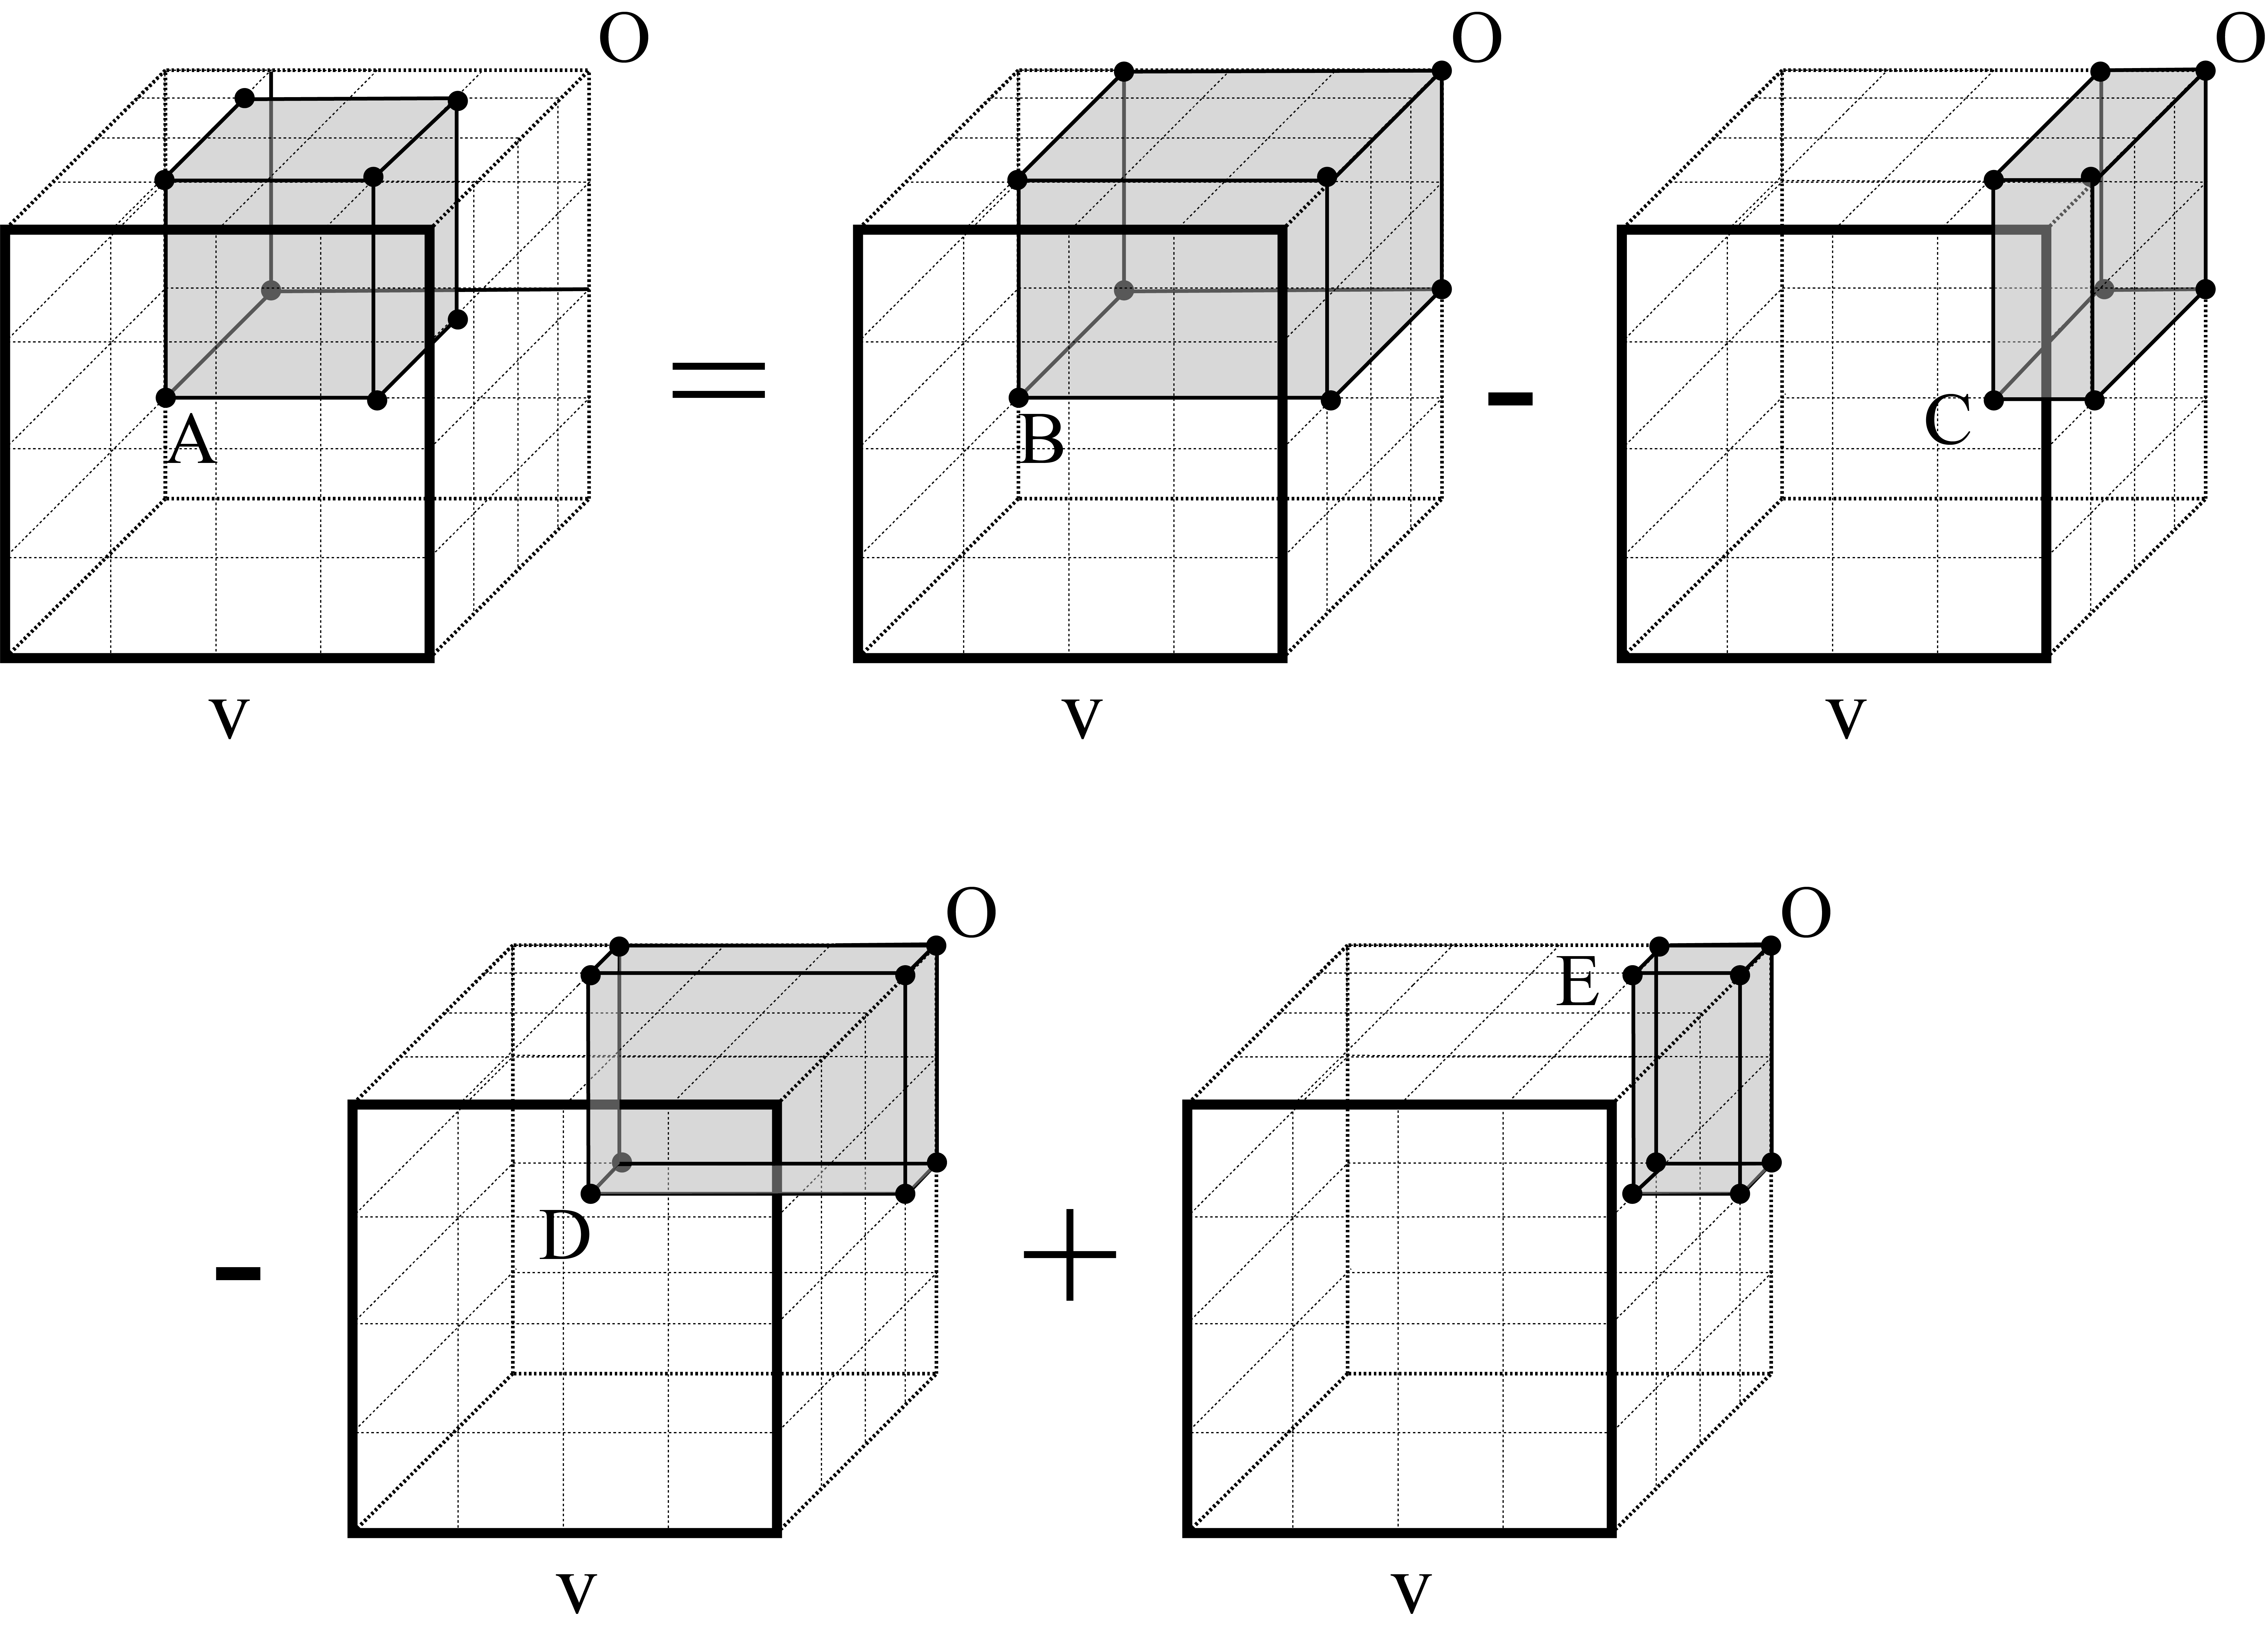
\includegraphics[width=0.45\textwidth]{figures/3D BIT.png}
Figure: Region query on 3D binary indexed tree  \\

The source code is published open source on github. Refer to our paper "Volume Computation of 3D Reconstructed Objects From Volumetric
Data Using Binary Indexed Tree"


\subsubsection{Coronary Artery Diameter Measurement}
\includegraphics[width=0.5\textwidth]{figures/sphere.png} \\
Figure: Diameter measurement of coronary arteries to estimate hypertenosis or stenosis. \\

Our Triple View R-Net is integrated into VasculAR software to partition volumetric cardiac data into number of semantically/anatomically meaningful regions, enabling the extraction of quantitative measures crucial for clinical assessment. With our algorithm, we can accurately measure myocardial wall thickness, providing invaluable support to radiologists and physicians in determining the presence of artery hypertenosis and evaluating myocardial health.

Our approach involves the utilization of a breadth-first search algorithm to efficiently identify neighboring vertices within the intricate 3D mesh when users interact with the spatial data. This method ensures a comprehensive exploration of the surrounding structures and facilitates precise measurements. Furthermore, we employ an interpolation technique to derive the center and radius of the most fitted sphere, enhancing the accuracy of our analyses. Through these advanced computational methods, we aim to revolutionize the process of cardiac analysis and empower medical professionals with enhanced diagnostic capabilities.


\subsection{Virtual Space Simulation \& Interaction}
By employing interactive programming within a virtual space using Unity, the team has created an environment enabling physicians to interactively manipulate and perform dissections on anatomical heart models directly. This solution surpasses the limitations of displaying 3D heart structures on flat screens, allowing users to delve into specific regions of the heart and interact with it in a flexible manner.

\subsubsection{3D Cardiac Structures Reconstruction}
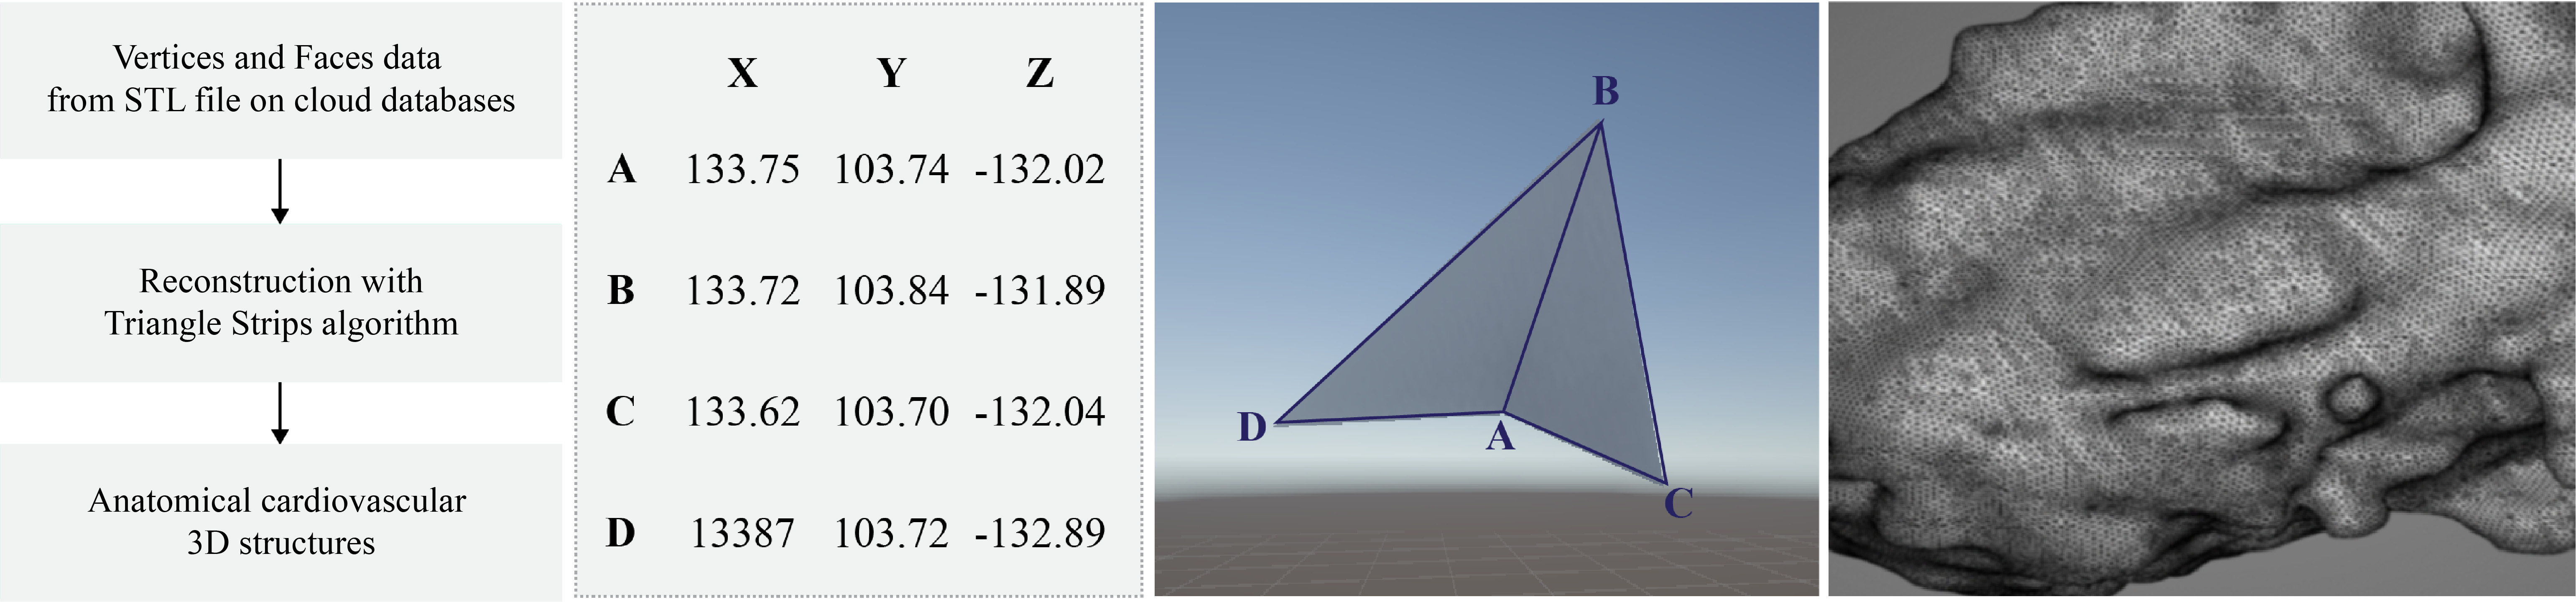
\includegraphics[width=0.49\textwidth]{figures/strip.png} \\
Figure: The process of calculating and reconstructing the structure of the heart. \\

The STL file contains a 3D mesh structure with coordinates (x, y, z) of 600,000 to 4,000,000 vertices. To reconstruct the 3D structure of the heart in the Unity virtual space, the research team arranged the triangular vertices to allow Unity to identify and build triangles according to the correct slice image. For instance, in Figure 15, they ordered the 4 vertices (A, B, C), (B, A, D) in the coordinate system and optimized the reconstruction process by utilizing the method of generating triangle strips (Hoppe, 1999) to reduce memory space complexity during model reconstruction.



\subsubsection{Symmetric Projection}

This method allows users to perform slicing and dissecting the structures in space accurately, without damaging other parts.

The equation of the plane $ (P) $ is given by:
$$ Ax + By + Cz + D = 0 $$

Consider $(P)$ as a plane with the equation as above. When using this plane to cut a part of the body, this plane intersects with surrounding parts at an infinite number of points $(x, y, z)$ that satisfy the equation of the plane $(P)$. Thus, we have developed a method called Symmetrical Projection. The equation $(P)$ has a normal vector $\vec{n}=(A, B, C)$ and cuts through point $O(a_o, y_o, z_o)$. From there, we get the vector of center $O$ called unit vector $\vec{i} = (x_i, y_i, z_i)$ such that $\vec{i} \perp \vec{n}$. Using vector $\vec{i}$, we project all points symmetrically on both sides. If one part is in contact with four sides, it is entirely inside the cut; otherwise, if not in contact with any side, it is completely outside and unaffected by cutting. Finally, to separate two parts on the cutting surface, we calculate the angle $\theta$ between the normal vector (color) and each point on the object to determine its position based on three cases of angle $\theta$.

\subsubsection{Slicing Plane Boundary Adjustment}
\includegraphics[width=0.5\textwidth]{figures/plane.png} \\

$$
\left\{ 
    \begin{array}{ll}
        \vec{ON} \parallel \vec{OM} \\
        d_{ON} = (x_N - x_O)^2 + (y_N - y_O)^2 + (z_N - z_O)^2 = \theta^2
    \end{array}
\right.   
$$
$$
\left\{ 
    \begin{array}{ll}
        (x_N, y_N, z_N) = k(x_M, y_M, z_M) \\
        (kx_M - x_O)^2 + (ky_M - y_O)^2 + (kz_M - z_O)^2 = \theta^2
    \end{array}
\right. 
$$

We have a plane $(P)$ with center $O(x_0, y_0, z_0)$ that is already known, and point $M(x_M, y_M, z_M)$ lies outside the known boundary. Point $M$ is determined by the principle of symmetrical projection from above. Doctors and experts can change the length/width of the cutting plane by modifying the parameter $\theta$, which essentially changes $OM$ to obtain a new length $ON$. By solving equation (*), we find $k$, which is the correlation coefficient between two vectors: $OM$ and $ON$. From here, we determine the coordinates of point $N(x_N, y_N, z_N)$ and a new plane with a length/width ratio of $20 = 20N$.

\subsection{Conclusion \& Discussion}




\newpage
\bibliographystyle{IEEEtran}
\bibliography{references}
\end{multicols}
\end{document}